\section{Techniki LIME i SHAP}
Zagadnienia uczenia maszynowego postrzegane są niekiedy jako tzw. czarne skrzynki. Przekonanie to wzięło się z tego że, o ile prostsze modele są łatwo interpretowalne dla człowieka, o tyle te bardziej skomplikowane nie dają już żadnych wskazówek jakie cechy okazały się być decydujące jeśli chodzi o podjęte przez wybrany algorytm decyzje. Z pomocą przychodzą nam techniki SHAP i LIME. Pozwalaja one na przybliżoną ocenę które z cech miały wpływ na wynik klasyfikacji.\\

\subsection{LIME (Local Interpretable Model-agnostic Explanations)}

Lokalne modele zastępcze to modele interpretowalne, które służą do wyjaśniania pojedynczych przewidywań modeli uczenia maszynowego działających jak "czarne skrzynki". Praca dotycząca lokalnych, agnostycznych względem modelu wyjaśnień interpretowalnych (LIME) proponuje konkretną implementację lokalnych modeli zastępczych. Modele zastępcze są trenowane w celu przybliżenia przewidywań leżącego u podstaw modelu "czarnej skrzynki". Zamiast trenować globalny model zastępczy, LIME skupia się na szkoleniu lokalnych modeli zastępczych, aby wyjaśnić indywidualne przewidywania.\\

Podejście jest dość intuicyjne. Najpierw zapominamy o danych treningowych i wyobrazamy sobie, że mamy tylko model "czarnej skrzynki", do którego możesz wprowadzać dane i otrzymywać przewidywania modelu. Możemy testować skrzynkę tak często, jak chcemy. Naszym celem jest zrozumienie, dlaczego model uczenia maszynowego dokonał pewnego przewidywania. LIME testuje, co dzieje się z przewidywaniami, gdy wprowadzasz do modelu uczenia maszynowego warianty swoich danych. LIME generuje nowy zestaw danych składający się z zakłóconych próbek i odpowiadających im przewidywań modelu "czarnej skrzynki". Na tym nowym zestawie danych a następnie trenuje model interpretowalny, który jest ważony przez bliskość próbek do analizowanego przypadku. Modelem interpretowalnym może być dowolny model z rozdziału o modelach interpretowalnych, na przykład Lasso lub drzewo decyzyjne. Nauczony model powinien być dobrą lokalną aproksymacją przewidywań modelu uczenia maszynowego, ale nie musi być dobrą aproksymacją globalną. Tego rodzaju dokładność nazywa się także lokalną wiernością.\\

Matematycznie, lokalne modele zastępcze z ograniczeniem interpretowalności można wyrazić następująco:\\

\begin{equation}
    {explanation}(x) = \arg\min_{g \in G} L(f, g, \pi_x) + \Omega(g)
\end{equation}

Model wyjaśniający dla instancji \( x \) to model \( g \) (np. model regresji liniowej), który minimalizuje stratę \( L \) (np. błąd średniokwadratowy), mierząc jak blisko wyjaśnienie jest do przewidywania oryginalnego modelu \( f \) (np. model xgboost), przy jednoczesnym zachowaniu niskiej złożoności modelu \( \Omega(g) \) (np. preferowanie mniejszej liczby cech). \( G \) to rodzina możliwych wyjaśnień, na przykład wszystkie możliwe modele regresji liniowej. Miara bliskości \( \pi_x \) definiuje, jak duże sąsiedztwo wokół instancji \( x \) rozważamy dla wyjaśnienia. W praktyce LIME optymalizuje tylko część straty. Użytkownik musi określić złożoność, np. wybierając maksymalną liczbę cech, które może użyć model regresji liniowej. \cite{lime}\\

LIME może być stosowany zarówno dla danych tabelarycznych, obrazów oraz tekstu.\\

\subsubsection{LIME dla danych tabelarycznych i klasyfikacji wieloklasowej}

Dane tabelaryczne to dane przedstawione w tabelach, gdzie każdy wiersz reprezentuje jedną instancję, a każda kolumna - cechę. Próbki LIME nie są pobierane wokół interesującej instancji, lecz z centralnej masy danych treningowych, co jest problematyczne. Jednakże zwiększa to prawdopodobieństwo, że wynik dla niektórych punktów próbki będzie różnił się od punktu danych, który nas interesuje (instancji), i że LIME będzie w stanie przynajmniej w pewnym stopniu wyjaśnić wynik klasyfikacji.\\

Dane użyte do wyjaśnienia techniką LIME nie powinny być normalizowane czy skalowane. Stanowi to pewnego rodzaju problem gdyż musimy budować nowy model (np. dla naiwnego klasyfikatora Bayesa) aby uniknąć pomyłki z tym bardziej optymalnym już znormalizowanym.\\

Po definicji explainera (w wolnym tłumaczeniu "wyjaśniacza"):

\begin{lstlisting}[caption=Definicja explainera]
#Stworz explainer z danych treningowych (potrzebuje surowych, 
                                         nieprzeskalowanych danych)
explainer = LimeTabularExplainer(
    training\_data=X\_train.values,  # nieprzeskalowane dane treningowe
    feature_names=df.columns[:-1].tolist(),  # nazwy cech
    class\_names=class\_labels,  # nazwy klas
    mode='classification'  # dla zadania klasyfikacji
)
\end{lstlisting}

Następnie wybieramy instancję do interpretacji (najcześciej definiujemy iterator wskazujący na numer instancji w zbiorze testowym) i otrzymujemy graficzne wyjaśnienie podjętej przez algorytm decyzcji:\\

\begin{figure}[H]
    \centering
    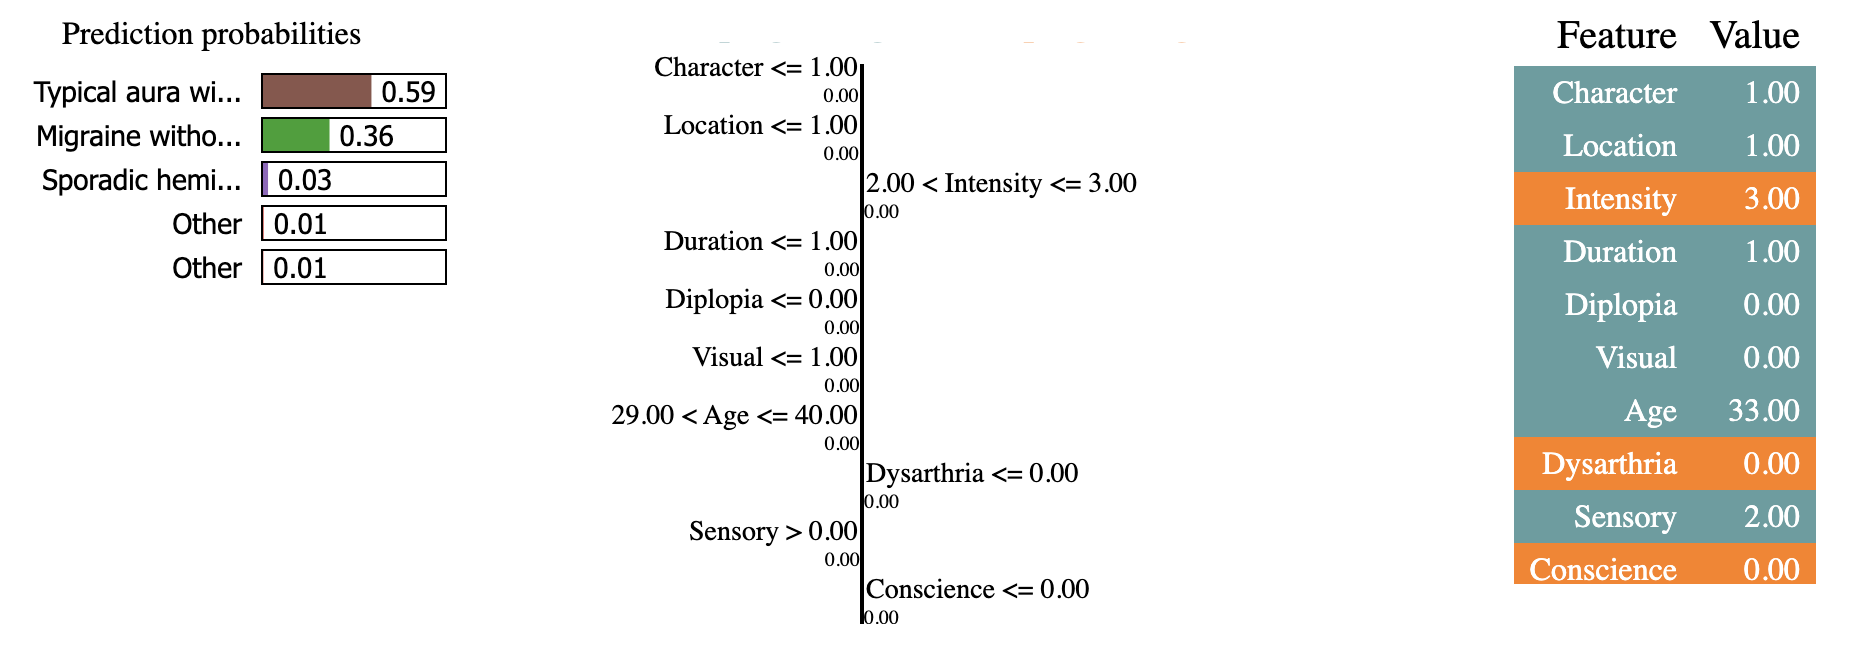
\includegraphics[scale=0.4]{lime_sin}
    \caption{Graficzna interpretacja decyzji modelu}
    \label{fig:lime_sin}
\end{figure}

Po stronie lewej widzimy tabelę podobieństwa do konkretnych klas. Po prawej wartości cech uszeregowane od najistotniejszych wg techniki LIME. Naj widzimy np. Po wartości wiersza "Age" dane nie są skalowane ani normalizowane. Na środku jest najistotniejszy element interpretacji, który akurat w naszym wypadku jest wyjątkowo nieczytelny ze względu na ograniczone możliwości skalowania osi. Natomiast istnieje jeszcze inna możliwość wyświetlenia tego wykresu:\\

\begin{figure}[H]
    \centering
    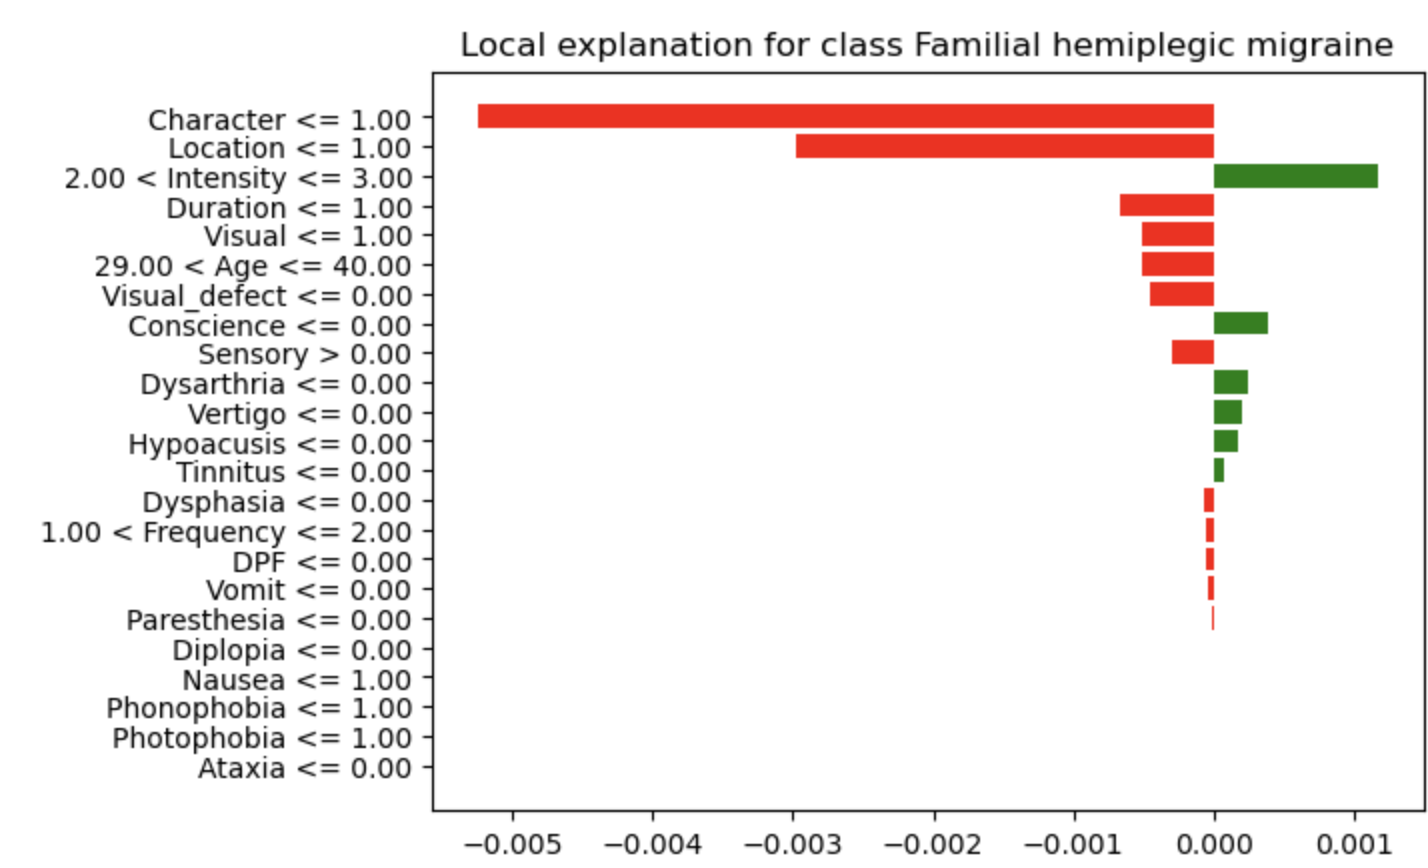
\includegraphics[scale=0.4]{lime_det}
    \caption{Szczegółowy wykres istotności cech}
    \label{fig:lime_det}
\end{figure}

Na osi pionowej widzimy nazwy cech wraz z przedziałami ich wartości dla analizowanej instancji. Na osi poziomej widzimy orientacyjną wartość na cecha ta wpływała na wynik - zarówno jeśli cecha świadczyła za przynależnością do klasy (wartości dodatnie oznaczone na zielono) jak i wpływ cech przeciw klasyfikacji (ujemne wartości oznaczone na czerwono). Dla czytelności wybrałem tabelę z innego przykładu. Widzimy jak pomiędzy obrazkiem nr \ref{fig:lime_det} pokrywają się cechy z lewej i prawej strony osi wobec tego widzimy skróconej interpretacji z obrazka nr \ref{fig:lime_sin}.

\subsection{SHAP (SHapley Additive exPlanations)}


Celem SHAP jest wyjaśnienie prognozy instancji $x$ poprzez obliczenie wkładu każdej cechy do prognozy. Metoda wyjaśniająca SHAP oblicza wartości Shapleya z teorii gier koalicyjnych. Wartości cech danej instancji danych działają jak gracze w koalicji. Wartości Shapleya mówią nam, jak sprawiedliwie rozdzielić „wypłatę” (= prognozę) między cechy. Graczem może być pojedyncza wartość cechy, np. dla danych tabelarycznych. Graczem może być także grupa wartości cech. Na przykład, aby wyjaśnić obraz, piksele można grupować w superpiksele i rozdzielić prognozę między nie. Jedną z innowacji, które wnosi SHAP, jest to, że wyjaśnienie wartości Shapleya jest przedstawiane jako addytywna metoda atrybucji cech, model liniowy. Ta perspektywa łączy LIME i wartości Shapleya. SHAP określa wyjaśnienie jako:

\[
g(z') = \phi_0 + \sum_{j=1}^M \phi_j z'_j
\]

gdzie $g$ to model wyjaśniający, $z' \in \{0,1\}^M$ jest wektorem koalicyjnym, $M$ to maksymalny rozmiar koalicji, a $\phi_j \in \mathbb{R}$ to atrybucja cechy dla cechy $j$, wartości Shapleya. To, co nazywam „wektorem koalicyjnym”, nazywane jest „uprościowymi cechami” w artykule SHAP. Myślę, że ta nazwa została wybrana, ponieważ np. dla danych obrazowych, obrazy nie są reprezentowane na poziomie pikseli, lecz agregowane do superpikseli. Uważam, że pomocne jest myślenie o $z'$ jako opisujących koalicje: w wektorze koalicyjnym, wpis 1 oznacza, że odpowiednia wartość cechy jest „obecna”, a 0, że jest „nieobecna”. To powinno brzmieć znajomo, jeśli znasz wartości Shapleya. Aby obliczyć wartości Shapleya, symulujemy, że tylko niektóre wartości cech biorą udział („obecne”), a niektóre nie („nieobecne”). Reprezentacja jako model liniowy koalicji to trik do obliczania $\phi$’s. Dla $x$, interesującej nas instancji, wektor koalicyjny $x'$ to wektor samych 1, tj. wszystkie wartości cech są „obecne”. Wzór upraszcza się do:

\[
g(x') = \phi_0 + \sum_{j=1}^M \phi_j
\]

Możesz znaleźć ten wzór w podobnej notacji w rozdziale o wartościach Shapleya. Więcej o faktycznej estymacji pojawi się później. Najpierw porozmawiajmy o właściwościach $\phi$’s, zanim przejdziemy do szczegółów ich estymacji.

Wartości Shapleya są jedynym rozwiązaniem, które spełnia właściwości Efektywności, Symetrii, Pomocniczości i Addytywności. SHAP również je spełnia, ponieważ oblicza wartości Shapleya. W artykule SHAP znajdziesz rozbieżności między właściwościami SHAP a właściwościami Shapleya. SHAP opisuje następujące trzy pożądane właściwości:\\

\textbf{Lokalna dokładność}

\[
\hat{f}(x) = g(x') = \phi_0 + \sum_{j=1}^M \phi_j x'_j
\]

Jeśli zdefiniujesz $\phi_0 = E_X(\hat{f}(x))$ i ustawisz wszystkie $x'_j$ na 1, to jest to właściwość efektywności Shapleya. Tylko z inną nazwą i używając wektora koalicyjnego.

\[
\hat{f}(x) = \phi_0 + \sum_{j=1}^M \phi_j x'_j = E_X(\hat{f}(X)) + \sum_{j=1}^M \phi_j
\]

\textbf{Brak wartości}

\[
x'_j = 0 \Rightarrow \phi_j = 0
\]

Brak wartości oznacza, że brakująca cecha otrzymuje atrybucję równą zero. Zauważ, że $x'_j$ odnosi się do koalicji, gdzie wartość 0 reprezentuje brak wartości cechy. W notacji koalicyjnej, wszystkie wartości cech $x'_j$ instancji, którą chcemy wyjaśnić, powinny być ‘1’. Obecność 0 oznaczałaby, że wartość cechy jest nieobecna dla interesującej nas instancji. Ta właściwość nie należy do właściwości „normalnych” wartości Shapleya. Więc dlaczego jej potrzebujemy dla SHAP? Lundberg nazywa to „drobnostką księgowości”. Brakująca cecha mogłaby – teoretycznie – mieć dowolną wartość Shapleya bez naruszania właściwości lokalnej dokładności, ponieważ jest mnożona przez $x'_j = 0$. Właściwość Brak wartości wymusza, aby brakujące cechy miały wartość Shapleya równą 0. W praktyce, jest to istotne tylko dla cech stałych.\\

\textbf{Spójność}\\

Niech $\hat{f}_x(z') = \hat{f}(h_x(z'))$ i $z'_{-j}$ oznacza, że $z'_j = 0$. Dla dowolnych dwóch modeli $f$ i $f'$, które spełniają:

\[
\hat{f}'_x(z') - \hat{f}'_x(z'_{-j}) \ge \hat{f}_x(z') - \hat{f}_x(z'_{-j})
\]

dla wszystkich wejść $z' \in \{0,1\}^M$, wtedy:

\[
\phi_j(\hat{f}',x) \ge \phi_j(\hat{f},x)
\]

Właściwość spójności mówi, że jeśli model zmienia się tak, że marginalny wkład wartości cechy wzrasta lub pozostaje taki sam (niezależnie od innych cech), wartość Shapleya również wzrasta lub pozostaje taka sama. Z właściwości Spójności wynikają właściwości wartości Shapleya: Liniowość, Pomocniczość i Symetria. \cite{shap} \\

\subsubsection{Zalety}

Ponieważ SHAP oblicza wartości Shapleya, wszystkie zalety wartości Shapleya mają zastosowanie: SHAP ma solidne teoretyczne podstawy w teorii gier. Prognoza jest sprawiedliwie rozdzielona między wartości cech. Otrzymujemy kontrastowe wyjaśnienia, które porównują prognozę z prognozą średnią. \cite{shap}\\

SHAP łączy LIME i wartości Shapleya. Jest to bardzo przydatne do lepszego zrozumienia obu metod. Pomaga to również w ujednoliceniu dziedziny interpretowalnego uczenia maszynowego. \cite{shap}\\

SHAP ma szybką implementację dla modeli drzewiastych. Uważam, że to klucz do popularności SHAP, ponieważ największą przeszkodą w przyjęciu wartości Shapleya jest wolne obliczanie. \cite{shap}\\

Szybkie obliczenia umożliwiają obliczanie wielu wartości Shapleya potrzebnych do globalnych interpretacji modelu. Globalne metody interpretacji obejmują znaczenie cech, zależność cech, interakcje, grupowanie i wykresy podsumowujące. Z SHAP globalne interpretacje są zgodne z lokalnymi wyjaśnieniami, ponieważ wartości Shapleya są „jednostką atomową” globalnych interpretacji. Jeśli używasz LIME do lokalnych wyjaśnień oraz wykresów częściowej zależności i permutacyjnej ważności cech do globalnych wyjaśnień, brakuje ci wspólnej podstawy. \cite{shap}\\

\subsubsection{Wady}

KernelSHAP jest powolny. To sprawia, że KernelSHAP jest niepraktyczny do użycia, gdy chcesz obliczyć wartości Shapleya dla wielu instancji. Ponadto wszystkie globalne metody SHAP, takie jak znaczenie cech SHAP, wymagają obliczenia wartości Shapleya dla wielu instancji. \cite{shap}\\

KernelSHAP ignoruje zależność cech. Większość innych metod interpretacji opartych na permutacji ma ten problem. Zastępując wartości cech wartościami z losowych instancji, zwykle łatwiej jest losowo próbować z rozkładu brzegowego. Jednak jeśli cechy są zależne, np. skorelowane, prowadzi to do nadania zbyt dużej wagi mało prawdopodobnym punktom danych. TreeSHAP rozwiązuje ten problem, explicity modelując warunkową prognozę oczekiwaną. \cite{shap}\\

Możliwe jest tworzenie celowo wprowadzających w błąd interpretacji z SHAP, które mogą ukrywać uprzedzenia. Jeśli jesteś naukowcem zajmującym się danymi, który tworzy wyjaśnienia, nie stanowi to problemu (byłoby to nawet zaletą, jeśli jesteś złym naukowcem danych, który chce tworzyć wprowadzające w błąd wyjaśnienia). Dla odbiorców wyjaśnienia SHAP jest to wada: nie mogą być pewni prawdziwości wyjaśnienia. \cite{shap} \\

Biblioteka SHAP umożliwia szereg interpretacji decyzyjności modeli. W naszym wypadku zachodziła jedynie konieczność interpretacji dla interpretacji użycia sieci głębokiej sieci neuronowej dla danych tabelarycznych i klasyfikacji wieloklasowej. Przykłady interpretacji dla analizowanego przypadku znajdują się w rodziale "Eksperymenty". Poniżej natomiast link do artykułu o podstawach interpretacji SHAP:\\
\url{https://miroslawmamczur.pl/wartosc-shapleya-interpretacja-modeli-blackbox/}
